% !TeX root = ..//fp_nmr_schmitt_kleinbek_18.tex

\thispagestyle{empty}
\frame{\titlepage}
\frame{\frametitle{Inhaltsübersicht}\tableofcontents}


%---------------
%Relaxationszeiten
%---------------
\section{Relaxationszeit}
\begin{frame}{Physikalischer Hintergrund}
	\begin{itemize}
	\item Teilchen mit Spin $S\neq 0$
	\item Energieaufspaltung durch parallele bzw. antiparallele Ausrichtung
		\begin{align*}
		\Delta E = -\vec{\mu}\cdot\vec{B}_0
		\end{align*}
	\item Resultierendes Drehmoment
		\begin{align*}
		\vec{\tau}=\vec{M}\times\vec{B}_0
		\end{align*}
	\end{itemize}
\end{frame}

\begin{frame}{Physikalischer Hintergrund}
	\begin{itemize}
	\item Rotation mit Larmorfrequenz
		\begin{align*}
		\omega_\text{L}=\gamma B_0
		\end{align*}
	\end{itemize}
	\begin{figure}
	% !TeX root = ..//f61_longreport_schmitt_kleinbek.tex
\begin{tikzpicture}[scale=.75]
\draw[arrows=-{Stealth[scale=.75]}, ultra thick, color=grey] (0,0)--+(0,4) node [above]{$B_0$};
\draw[arrows=-{Stealth[scale=.75]}, line width=1mm, color=myred] (0,0)--+(0,2) node [left]{$M$};
\fill (0,0) circle (1.9pt)[color=myred];

\draw [thick, rotate=-23](3.7,3.43) ellipse (.8cm and .4cm);
\draw[arrows=-{Stealth[scale=.75]}, ultra thick, color=grey] (4,0)--+(0,4) node [above]{$B_0$};
\draw[arrows=-{Stealth[scale=.75]}, ultra thick, color=grey, dashed] (4,0)--+(1.5,0) node [below]{$B_1$};
\draw[arrows=-{Stealth[scale=.75]}, line width=.75mm] (4,0)--+(1.5,4) node [right]{$B_\text{tot}$};
\draw[arrows=-{Stealth[scale=.75]}, line width=1mm, color=myred] (4,0)--+(0,2) node [left]{$M$};
\fill (4,0) circle (1.9pt)[color=myred];

\draw [thick, rotate=18](11.3,-2.8) ellipse (1.9cm and .4cm);
\draw[arrows=-{Stealth[scale=.75]}, ultra thick, color=grey] (12,0)--+(0,4) node [above]{$B_0$};
\draw[arrows=-{Stealth[scale=.75]}, ultra thick, color=grey, dashed] (12,0)--+(-1.5,0) node [below]{$B_1$};
\draw[arrows=-{Stealth[scale=.75]}, line width=.75mm] (12,0)--+(-1.5,4) node [left]{$B_\text{tot}$};
\draw[arrows=-{Stealth[scale=.75]}, line width=1mm, color=myred] (12,0)--+(45:2) node [right]{$M$};
\fill (12,0) circle (1.9pt)[color=myred];
\end{tikzpicture}
	\caption{Auslenkung der Magnetisierung}
	\end{figure}
\end{frame}

\begin{frame}{Physikalischer Hintergrund}
$\Rightarrow$ \SI{90}{\degree} und \SI{180}{\degree} Pulse durch Veränderung
	\begin{itemize}
	\item Messung der Ausrichtung der Magnetisierung durch Induktion
	\item Zerfall der Magnetisierung
	\begin{align*}
	M_\parallel (t)&=M_0\left(1-2\cdot\e{-\frac{t}{T_1}}\right)\\
	M_\bot(t)&=M_0\cdot\e{-\frac{t}{T_2}}
	\end{align*}
	\end{itemize}
	\begin{block}{Ursache}
	parallel: Spin-Gitter-WW\\
	antiparallel: Spin-Spin-WW
	\end{block}
\end{frame}

\begin{frame}{Spin-Echo-Methode}
Messung der Spin-Gitter Relaxationszeit $T_1$
	\begin{figure}
	\centering
	% !TeX root = ..//fp_nmr_schmitt_kleinbek_18.tex
\begin{tikzpicture}[scale=.7]
%point
\foreach \i in {4.5,9}
\fill (\i,0) circle (2pt);

%circle
\foreach \i in {0,4.5,9,13.5}
\draw [thick] (\i,0) circle (1cm);

%time
\node at (0,2.5){$t=0$};
\node at (4.5,2.5){$t=\tau$};
\node at (9,2.5){$t=\tau$};
\node at (13.5,2.5){$t=2\tau$};
\node at (1.2,1.25)[color=grey]{$\ang{90}$-Puls};

%coordinates
\foreach \i in {0,4.5,9,13.5}
\draw[arrows=-{Stealth[scale=1]},thick](\i,0)--+(0,1.5) node[left]{$x$};
\foreach \i in {0,4.5,9,13.5}
\draw[arrows=-{Stealth[scale=1]},thick](\i,0)--+(1.5,0) node[below]{$y$};

%timearrows
\draw[arrows=-{Stealth[scale=.75]}, color=grey, line width=.75mm](2,0)--+(1,0) node[midway, above]{$\tau$};
\draw[arrows=-{Stealth[scale=.75]}, color=grey, line width=.75mm](6.5,0)--+(1,0) node[midway, above]{$\ang{180}$};
\draw[arrows=-{Stealth[scale=.75]}, color=grey, line width=.75mm](11,0)--+(1,0) node[midway, above]{$\tau$};

%arrows
\draw[arrows=-{Stealth[scale=.5]}, color=myred, line width=1.25mm](0,0)--+(1.2,0) node[midway, below, xshift=-3pt]{\footnotesize $M_\bot$};
\draw[arrows=-{Stealth[scale=.5]}, color=myred, line width=1.25mm](13.5,0)--+(-1.2,0) node[midway, below, xshift=3pt]{\footnotesize $M_\bot$};
\draw[arrows=-{Stealth[scale=1]},thick](4.5,0)--+(-35:1.5) node[below]{$\omega_2$};
\draw[arrows=-{Stealth[scale=1]},thick](4.5,0)--+(-60:1.5) node[below]{$\omega_1$};
\draw[arrows=-{Stealth[scale=1]},thick](9,0)--+(215:1.5) node[below]{$\omega_2$};
\draw[arrows=-{Stealth[scale=1]},thick](9,0)--+(240:1.5) node[below]{$\omega_1$};

\draw[arrows=-{Stealth[scale=1]},thick, shift = {(0.8,-0.8)}](5.42,-.4) arc (-25:-80:1);
\draw[arrows=-{Stealth[scale=1]},thick, shift = {(-0.8,-0.8)}](8.8,-.97) arc (-100:-155:1);

%redcircle
\foreach \i in {0,13.5}
\fill (\i,0) circle (1.775pt)[color=myred];
\end{tikzpicture}
	\caption{Spin-Echo-Methode}
	\end{figure}
\end{frame}

\begin{frame}{Carr-Purcell-Methode}
Messung der Spin-Gitter Relaxationszeit $T_1$ und der Spin-Spin Relaxationszeit $T_2$
	\begin{figure}
	\centering
	%\input{images//carrpurcell.png}
	\caption{Carr-Purcell-Methode}
	\end{figure}
\end{frame}

\begin{frame}{Versuchsaufbau}
	\begin{figure}
	\centering
	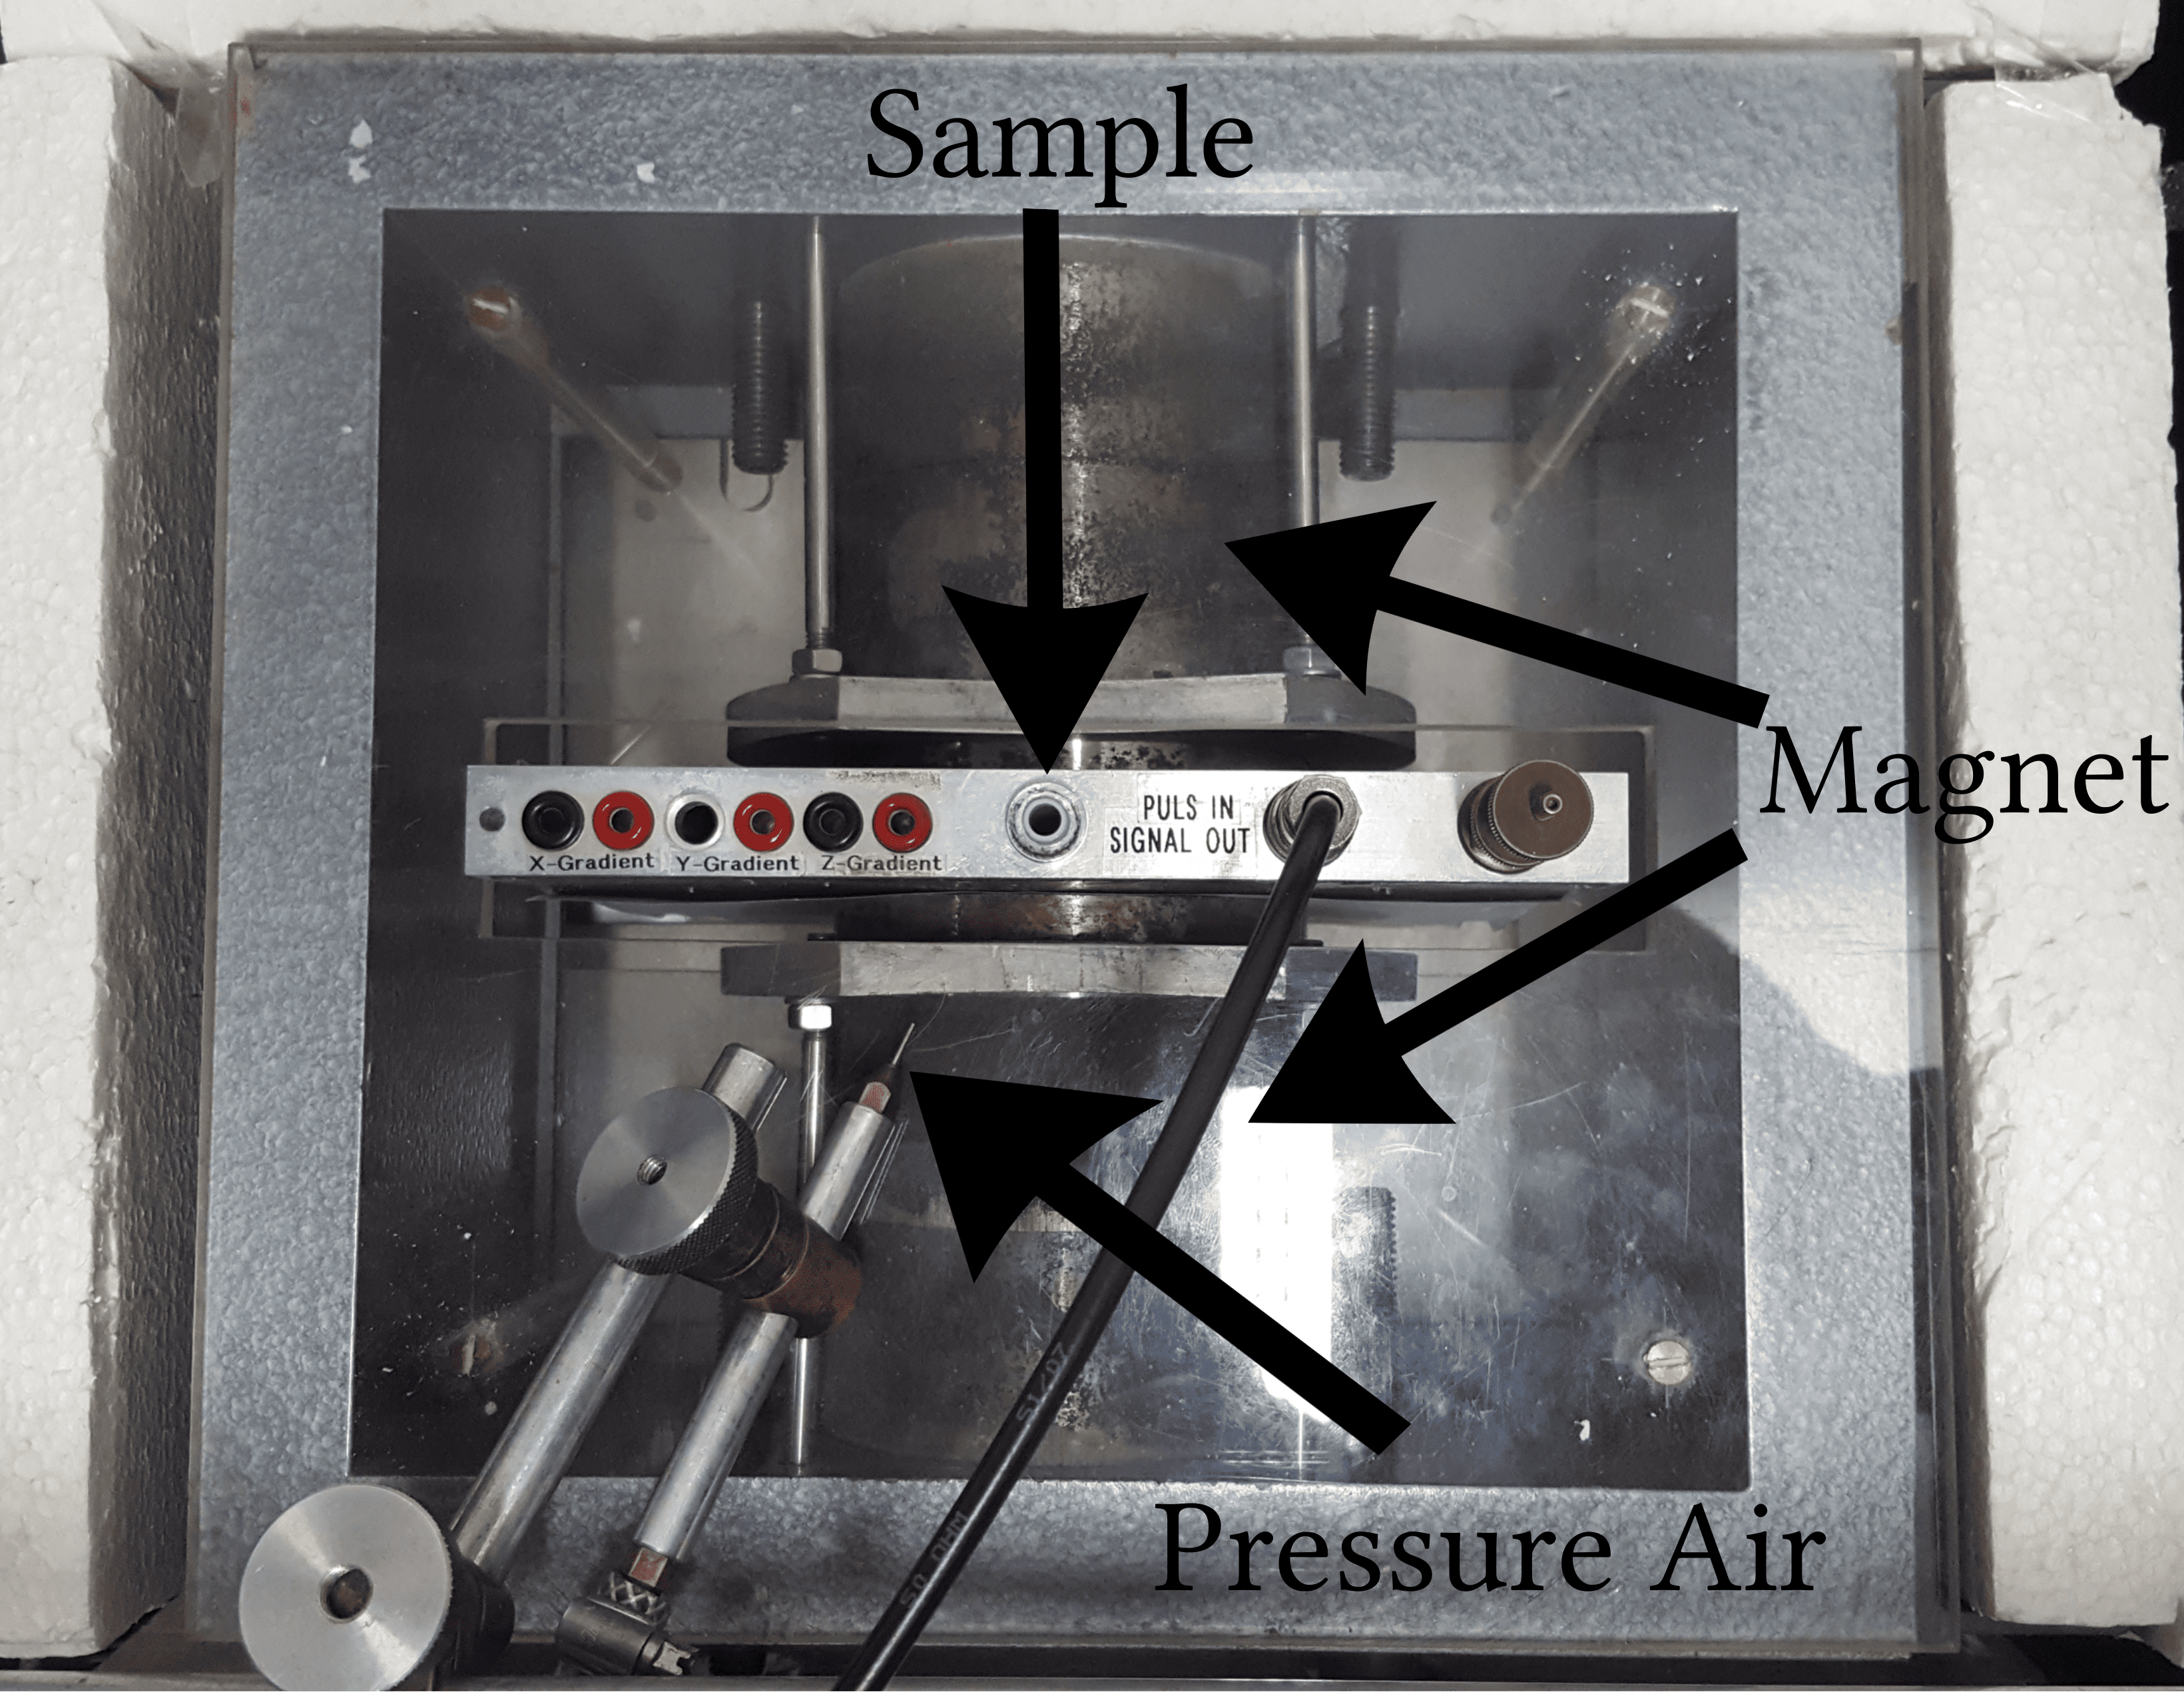
\includegraphics[scale=.075]{images//magnet.png}
	\caption{Magnet}
	\end{figure}
\end{frame}

\begin{frame}{Messung}
	\begin{align*}
	M_\parallel (t)&=M_0\left(1-2\cdot\e{-\frac{t}{T_1}}\right)
	\end{align*}
	\begin{figure}
	\centering
		\begin{subfigure}{.49\textwidth}
		\centering
		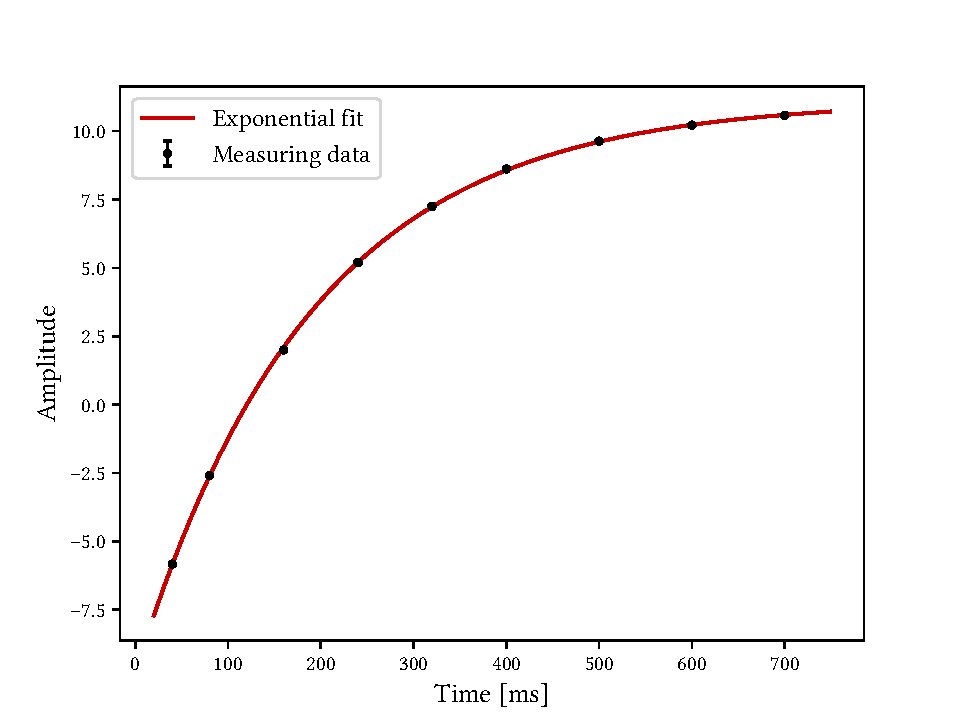
\includegraphics[scale=.36]{..//figures//f61_abb_1.pdf}
		\caption{Gd 500}
		\end{subfigure}
		\begin{subfigure}{.49\textwidth}
		\centering
		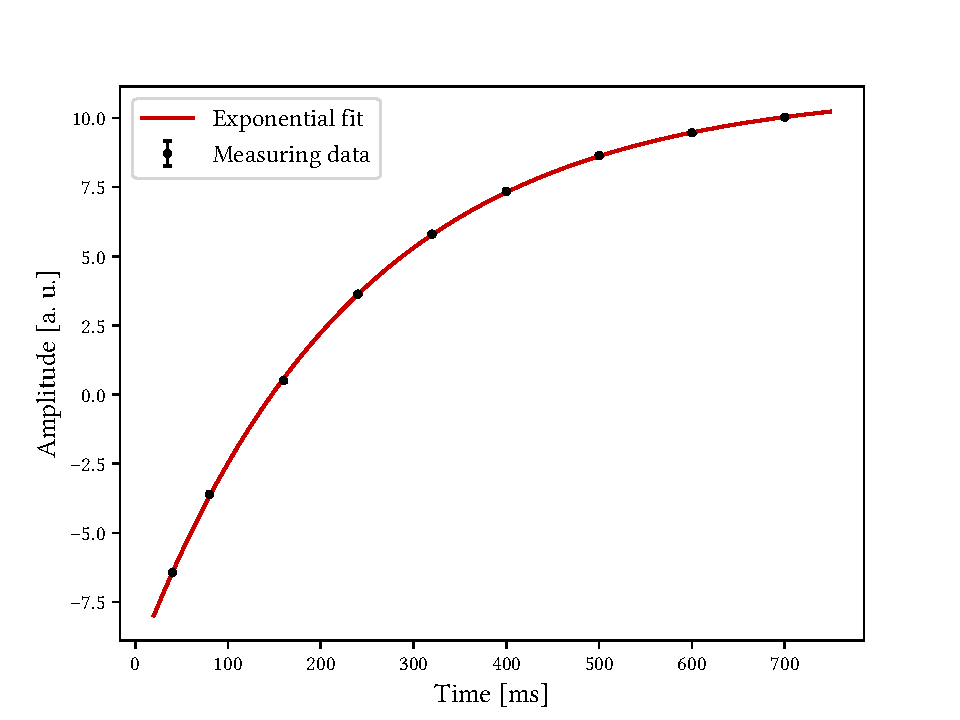
\includegraphics[scale=.36]{..//figures//f61_abb_1_600.pdf}
		\caption{Gd 600}
		\end{subfigure}
	\caption{Relaxationszeit $T_1$}
	\end{figure}
\end{frame}

\begin{frame}{Messung}
	\begin{align*}
	M_\bot(t)&=M_0\cdot\e{-\frac{t}{T_2}}
	\end{align*}
	\begin{figure}
	\centering
		\begin{subfigure}{.49\textwidth}
		\centering
		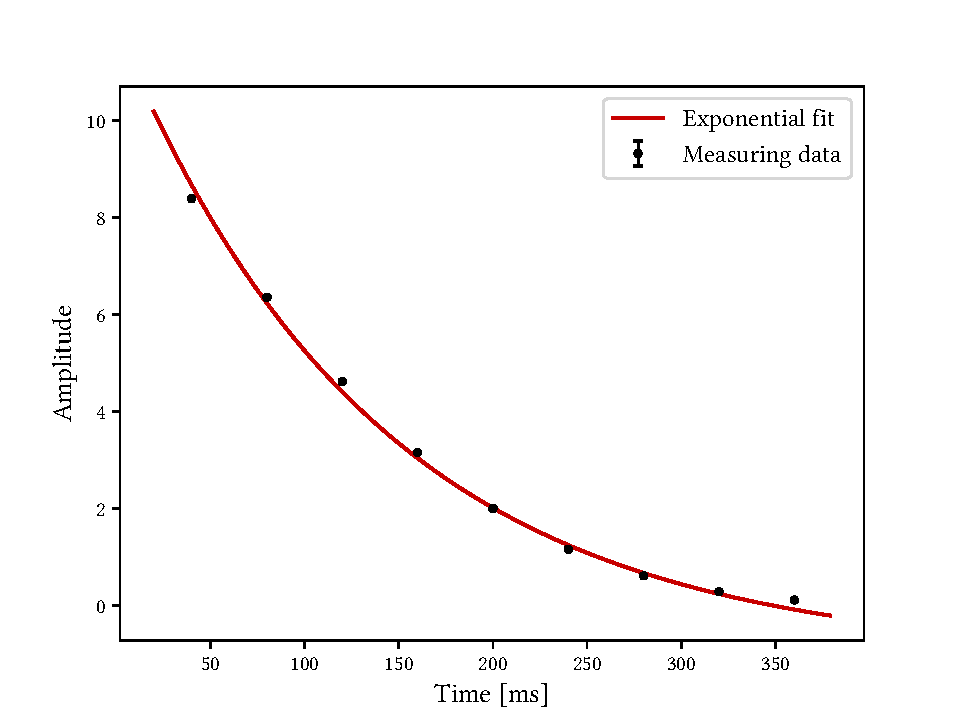
\includegraphics[scale=.36]{..//figures//f61_abb_2.pdf}
		\caption{Gd 500}
		\end{subfigure}
		\begin{subfigure}{.49\textwidth}
		\centering
		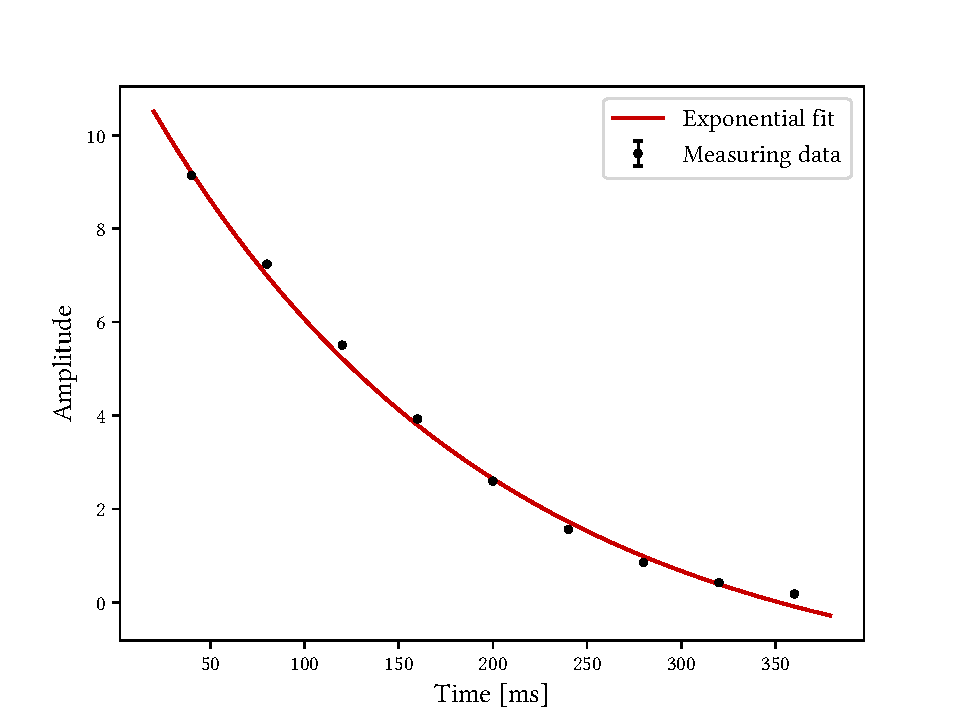
\includegraphics[scale=.36]{..//figures//f61_abb_2_600.pdf}
		\caption{Gd 600}
		\end{subfigure}
	\caption{Relaxationszeit $T_2$}
	\end{figure}
\end{frame}

\begin{frame}{Ergebnisse}
	\begin{table}
	\centering
	\begin{tabular}{cccc}
	\toprule
	Sample & $T_1$ [ms] & $T_{2,\text{ Spin-Echo}}$ [ms] & $T_{2,\text{ Carr-Purcell}}$ [ms]\\
	\midrule
	Gd500 & \num{190.0(6)} & \num{154.2(9)} & \num{170.1(4)}\\
	Gd600 & \num{234.3(5)} & \num{186.5(9)} & \num{198.2(7)}\\
	\bottomrule
	\end{tabular}
	\caption{Gemessene Relaxationszeiten}
	\end{table}
	\begin{block}{Ergebnis}
	\begin{itemize}
	\item $T_\text{Gd500} < T_\text{Gd600}$
	\item $T_2 < T_1$
	\item $T_\text{Spin-Echo} < T_\text{Carr-Purcell}$
	\end{itemize}
	\end{block}
\end{frame}




%---------------
%Chemical Shift
%---------------
\section{Chemische Verschiebung}
\begin{frame}{Physikalischer Hintergrund}
\begin{exampleblock}{alles}
hallo
\end{exampleblock}
\end{frame}





%---------------
%Bildgebung
%---------------
\section{Bildgebende Verfahren} %2D- und 3D-Bildgebung
\begin{frame}{Physikalischer Hintergrund}
\begin{figure}
\centering
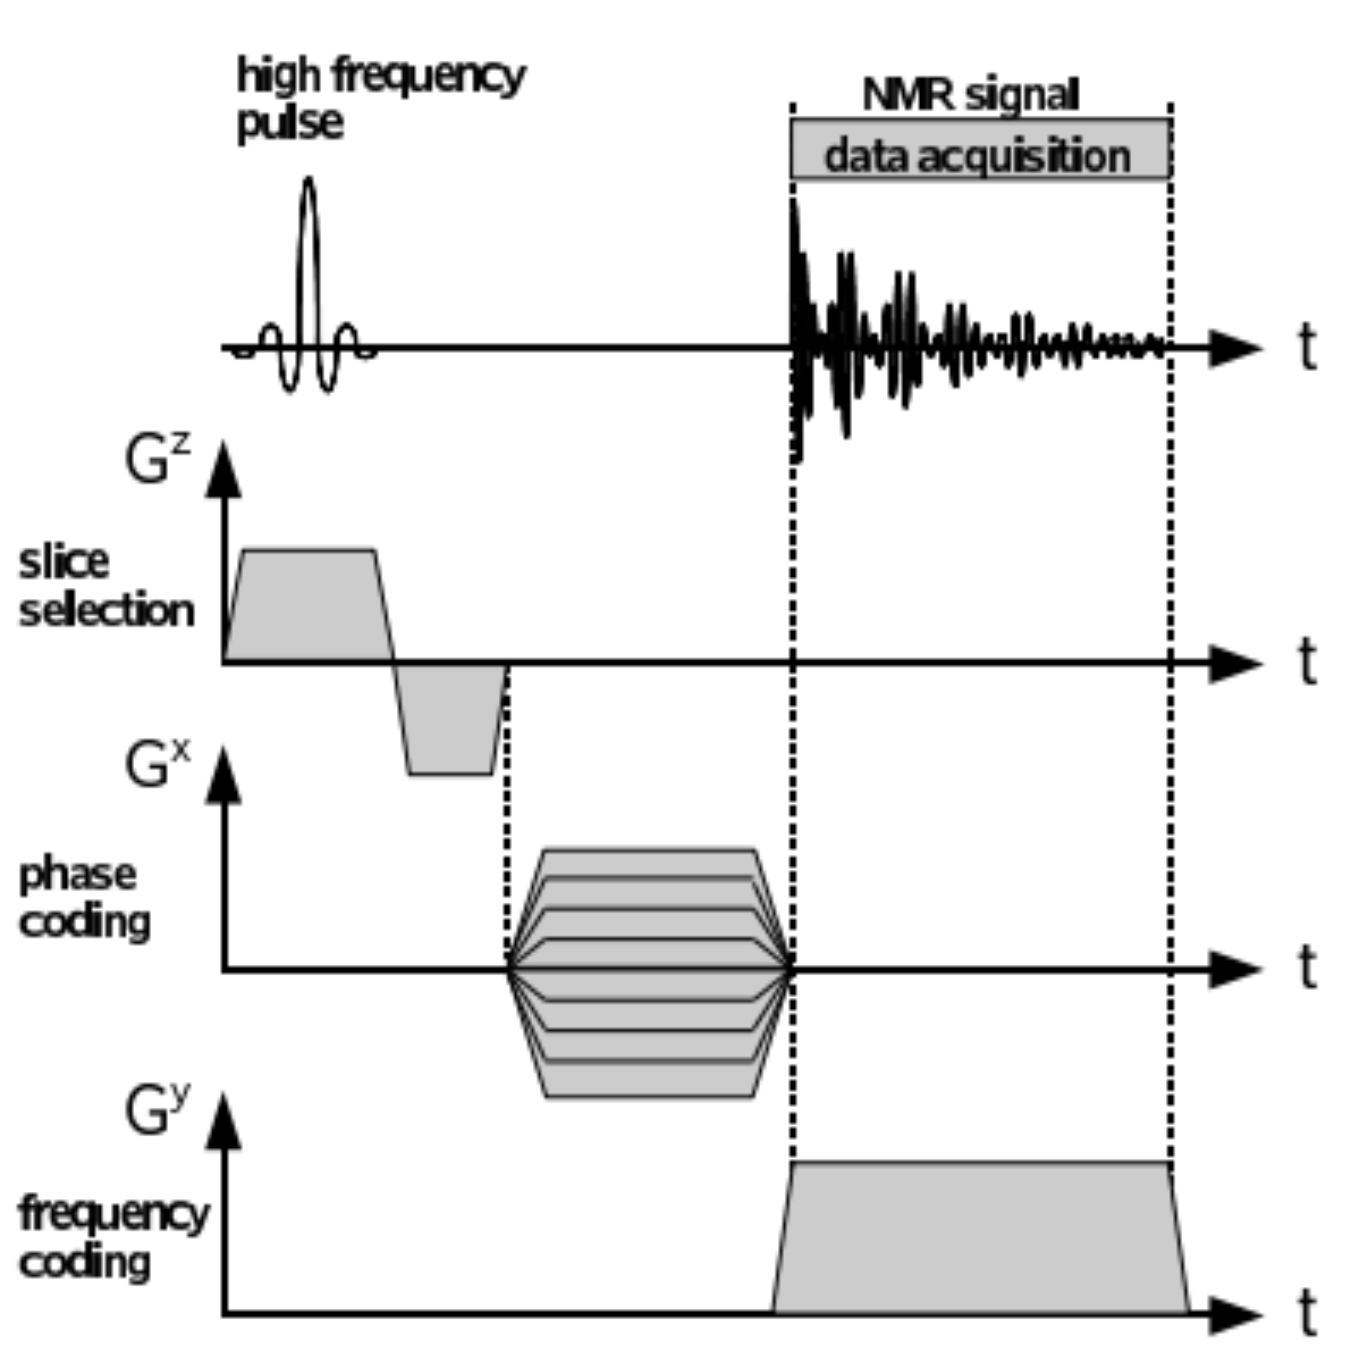
\includegraphics[scale=.1]{images//signal.png}
\caption{signal}
\end{figure}
\end{frame}




%---------------
%Diskussion
%---------------
\section{Diskussion}
\begin{frame}{Fazit}
	\begin{alertblock}{Contra}
	\begin{itemize}
	\item inhomogener Magnet
	\item Temperaturschwankungen
	\end{itemize}
	\end{alertblock}
	\begin{exampleblock}{Pro}
	\begin{itemize}
	\item nmr bei altem Gerät
	\item bilder
	\end{itemize}
	\end{exampleblock}
\end{frame}

\begin{frame}{Anwendung}
haehd
\end{frame}